%!TEX root = ../thesis.tex
%*******************************************************************************
%*********************************** First Chapter *****************************
%*******************************************************************************

\chapter{Introduction}  %Title of the First Chapter
\label{Introduction}

\ifpdf
    \graphicspath{{Chapter1/Figs/Raster/}{Chapter1/Figs/PDF/}{Chapter1/Figs/}}
\else
    \graphicspath{{Chapter1/Figs/Vector/}{Chapter1/Figs/}}
\fi
\section{Background}
Climate change has been a well-known problem among scientists for a long time. The first paper warning the effects of the increment of carbon dioxide in the atmosphere is from 1976 \cite{manabe_thermal_1967} while in a study of 1976 \cite{keeling_atmospheric_1976} they observed it for the first time. In 1988, the World Meteorological Organization Established the Intergovernmental Panel On Climate Change (IPCC) \cite{baker_1989}, which is up to date as the leading organization evaluating climate change. As shown in \cite{santos_climate_2021}, the researcher's interest in climate change grew significantly after 1990. 

\begin{figure}[H]
    \centering
    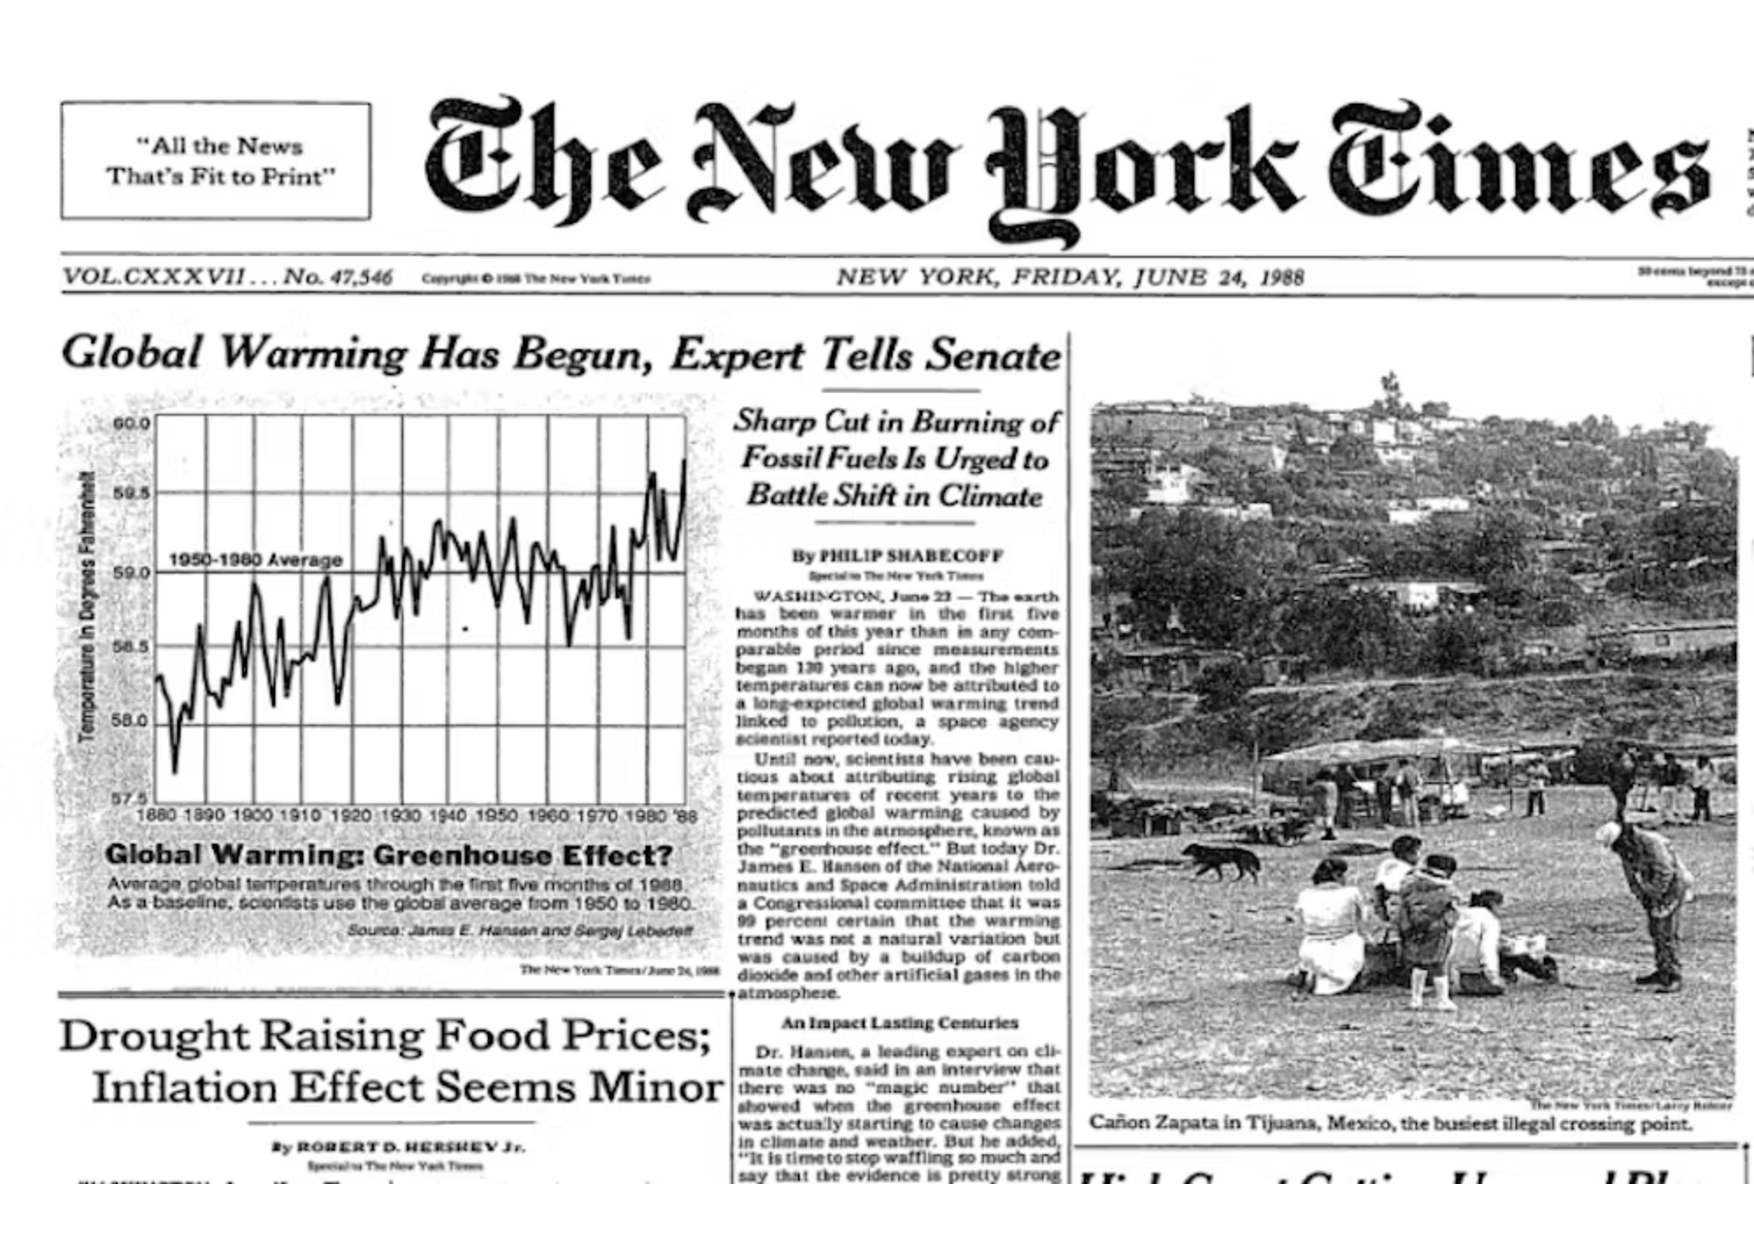
\includegraphics[width=0.75\linewidth]{Chapter1/figures/global_warming copy.pdf}
    \caption{Front page of NY Times, June 24, 1988 }
    \label{fig:enter-label}
\end{figure}

Only in the past few years has it become mainstream, in part thanks to Greta Thunberg \cite{sabherwal_greta_2021} and Fridays for Future, people were more aware of the problem. As we can see in Fig \ref{fig:google_greta}, only after 2019 people started searching (and talking) about a 'climate crisis' \footnote{we choose this term because it is not descriptive as climate change but has the negative version of it}, underlining the urgency with which we should act. It is also true that the strikes caused inconvenience to many normal citizens trying to go to their workplaces. This means that someone may have developed a bad feeling toward this activism and, thus, toward climate change. An increase in polarization has been detected after the strikes \cite{Falkenberg_climate_2022}.
\\


\begin{figure}
    \centering
    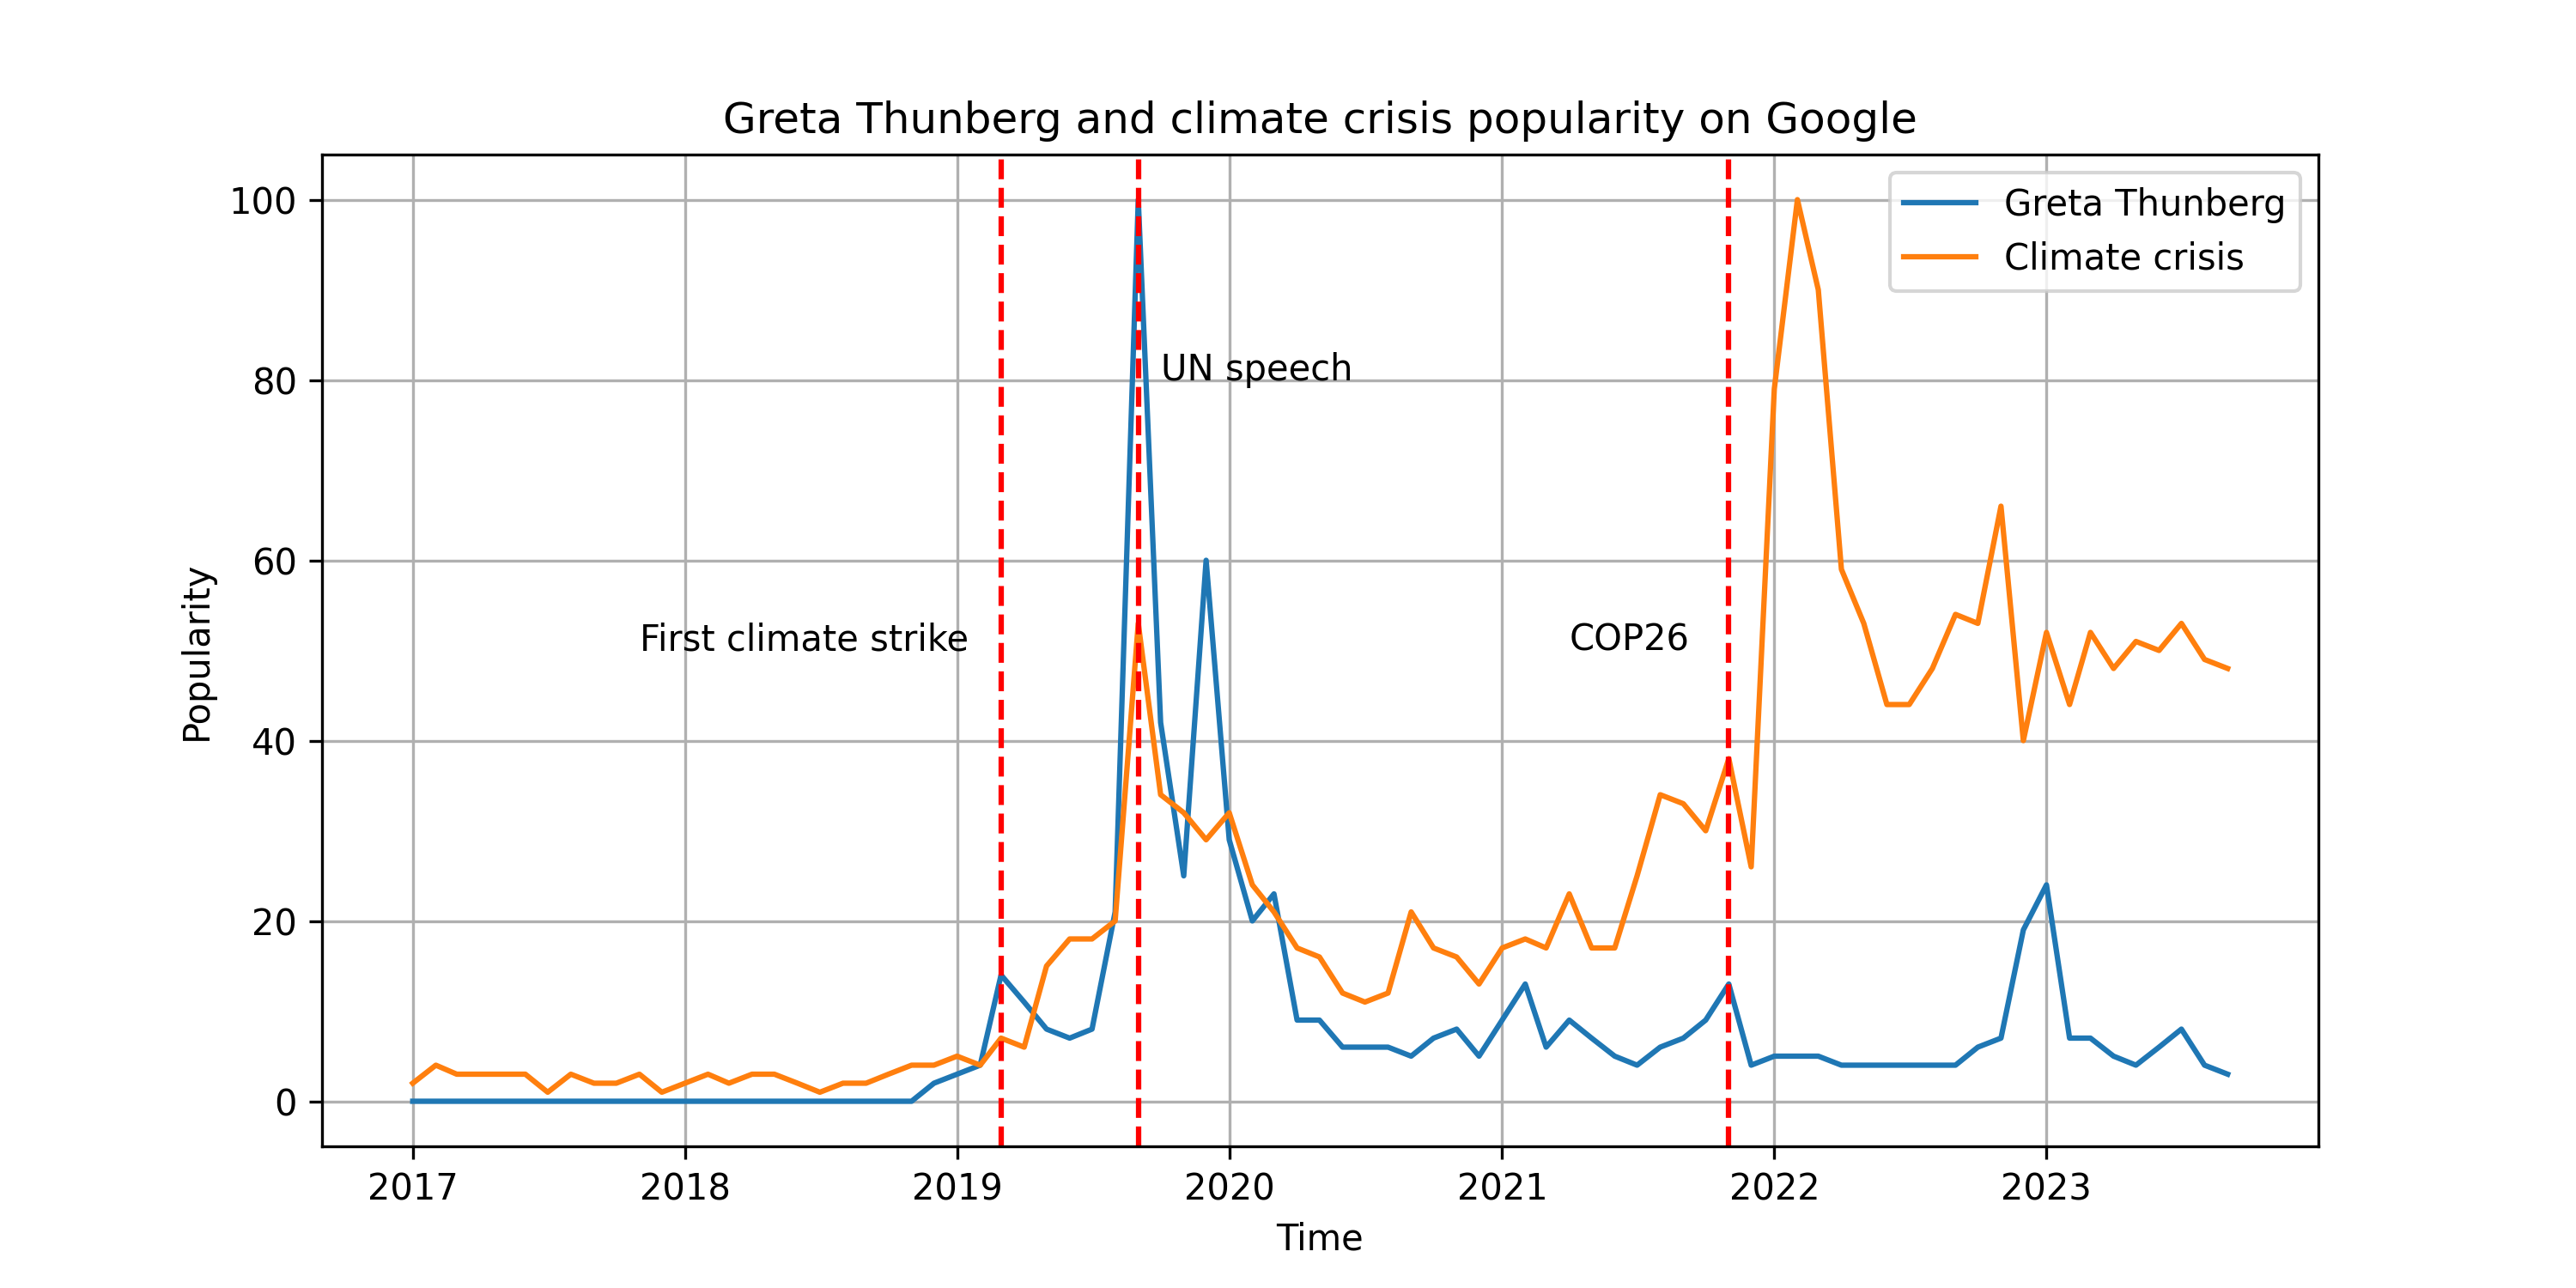
\includegraphics[width=0.85\linewidth]{Chapter1/figures/greta_climate_crisis.png}
    \caption{interest on Google over the time of Greta Thunberg and climate crisis}
    \label{fig:google_greta}
\end{figure}
In particular, Twitter is a place where political debate takes place \cite{Pew_twitter_2022} and political events like 
Conferences of Parties (COP) are the perfect opportunity to study climate change discussion because they are the conferences where the highest political figures of many countries meet and talk about climate emergencies. The increasing polarization poses a significant challenge to mitigating the harmful impacts of climate change; for this reason, understanting the root cause has the potential to contribute significantly to safeguarding the world from the impacts of climate change.



\paragraph{Conference of Parties}
Conferences of Parties are yearly conferences organized by the United Nations where the topic of discussion is climate change; the first was held in 1995 in Berlin, and the ones that ended with a document to ratify are:
\begin{itemize}
    \item \textbf{COP3}: Kyoto Protocol (1997) It was the first treaty to mandate countries to cut greenhouse gas emissions legally, but this was true only for developed countries, excluding China and India.
    \item \textbf{COP21}: The Paris Agreement (2015) is a global accord that aims to limit global warming to well below 2 degrees Celsius, preferably to 1.5 degrees Celsius, compared to pre-industrial levels by requiring all countries to set their own emissions reduction targets. It is considered more effective and inclusive than the Kyoto Protocol because it involves all countries, allows for flexibility in setting emissions targets, and includes a robust system for transparency and accountability.
    \item \textbf{COP26}: Glasgow Climate Pact (2021) is a crucial agreement in the global effort to combat climate change. It includes significant commitments to address the urgent challenges of climate change, such as phasing down coal usage, increasing climate finance for adaptation, strengthening international cooperation, and supporting countries in transitioning to low-carbon economies. However, not everyone agrees with the outcomes of the conference. \cite{arora_cop26_2021} \cite{layna_promises_2022} \cite{suresh_climate_2021}
\end{itemize}

\\
The focus of this work will be on cop26 which is the one that happened in a context of popular agitation toward the topic. Then a comparison with cop21 will be done due to its analogies with cop26, an important document has been ratified, the paris agreement, and then trump withdraw 


This work lays its foundations on the research of Falkenberg et al. \cite{falkenberg_growing_2022}, where they discovered that cop26 was way more polarized than cop21. Using a similar approach, we will explore the ideological polarization topic by topic. 

There is not a universally agreed definition of polarization. In this paper, we will use the one stated in \cite{bramson_understanding_2017}, the same used by Falkenberg, which is: "The most common measure of polarization in the political literature is probably bimodality, which is the idea that the population can be usefully broken down into two subpopulations". 
In our case, the two sub-populations are pro-climate and climate skeptics.



\section{Research Questions}
Thanks to the structure we gave to our research, we can now answer a new set of questions related to intra-topic polarization. The first and most straightforward is RQ1, which aims to inspect the topics that are driving the polarization of the entire COP26. Consequently, RQ2 wants to identify whether these topics have always been polarized.

Then, we will move to some questions related to the users; in particular, RQ3 wants to see if the polarized users are polarized in the same way over the different topics or if there are topics in which they are on the opposite side of the spectrum. RQ4 instead investigates whether the users who talk about many different topics are more polarized than those who are present in only one.



\begin{enumerate}
    \item  Which are the most polarizing topics discussed on Twitter during Cop 26?
    \item How did topics evolve between cop21 and cop26?
    \item Is the single-user polarization different across different topics? 
    \item Are the users present in more topics polarized in different ways than the ones that are present only in one or few topics?

\end{enumerate}






%********************************** %First Section  **************************************

\nomenclature[z-DEM]{DEM}{Discrete Element Method}
